\scanpage{32}\mspage{31}
% @ top, continuation lines 1–3
Si $A\in F\setminus G$, $A\cap B$ est réunion de strates de $F$. \deleted{Reste} reste à voir que une strate \inserted{\unsure{$G$|$\in$}} de $F$ est réunion de strates de $F'$. Soit $A$ cette strate de $F$. \deleted{\unsure{On}}
% @ top, cancelled union; the lower limit is literally F
\[
 \deleted{A=\bigcup_{\substack{B\in F\\B\leq F}}B^\circ}
\]
% @ upper part, two cases; both first-case G primes are visible
% Supplemental recheck: separate two-stroke hooked/arrow-like mark is drawn beneath the set-difference slash. Its function is unresolved.
Si $A\notin G'$, alors $A\in F\mathbin{\underset{\text{\begin{tikzpicture}[x=.25cm,y=.25cm]
\draw[line width=.45pt,line cap=round,line join=round] (.18,.43) -- (0,.05) -- (.15,.02);
\draw[line width=.45pt,line cap=round,line join=round] (.30,.60) .. controls (.36,.40) and (.26,.18) .. (.10,.04);
\end{tikzpicture}}}{\setminus}}G'\subset F'$, et on gagne. Si $A\in G$, alors (comme $G'\preceq G$) $A$ est réunion de strates de $G'$, qui sont des strates de $F'$, et on gagne encore.

% @ left beside corollary
% slanted
\margin{Ultra faux}
% @ upper middle, corollary heading
\uline{Corollaire} Le \deleted{raffinement}\inserted{subdivision} précédente $F'$ de $F$ est caractérisée par \inserted{chacune} des propriétés équivalentes suivantes~:

% @ centre, condition a), cancelled by a large cross
\figure{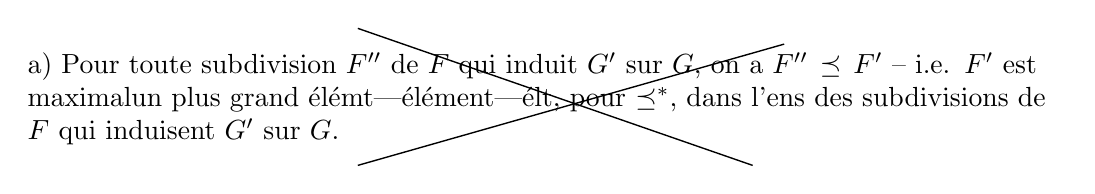
\begin{tikzpicture}[x=1cm,y=1cm]
\node[anchor=north west,inner sep=0pt,text width=13.2cm,align=left] (conditiona) at (0,0) {\deleted{a) Pour toute subdivision $F''$ de $F$ qui induit $G'$ sur $G$, on a $F''\preceq F'$ -- i.e. $F'$ est \deleted{\uline{maximal}}\inserted{un plus grand \unsure{élémt|élément|élt}}, pour $\preceq^{*}$, dans l'ens des subdivisions de $F$ qui induisent $G'$ sur $G$.}};
\draw[line width=.5pt] ([xshift=4.2cm,yshift=.3cm]conditiona.north west) -- ([xshift=-4.0cm,yshift=-.25cm]conditiona.south east);
\draw[line width=.5pt] ([xshift=4.2cm,yshift=-.25cm]conditiona.south west) -- ([xshift=-3.6cm,yshift=.1cm]conditiona.north east);
\end{tikzpicture}}
% @ within the crossed a), below qui: isolated angular pen mark.
% Identity unresolved (E / membership-like mark); these strokes are not assigned a textual role.
\figure{
\begin{tikzpicture}[x=1cm,y=1cm]
\draw[line width=.7pt] (0,.48) -- (.02,.03) .. controls (.10,-.02) and (.22,.01) .. (.42,.02);
\draw[line width=.65pt] (.13,.16) .. controls (.25,.22) and (.34,.22) .. (.47,.20);
\draw[gray,line width=.3pt] (.08,.47) .. controls (.21,.50) and (.35,.48) .. (.43,.44);
\draw[line width=.5pt] (.37,.73) -- (.43,.57);
\end{tikzpicture}}
% @ left of a), starred gloss
% slanted
\margin{$*$ ou pour $\ll$, cela revient au $=$ parmi des subdivisions d'une $=$ $F$}
% @ centre left, long oblique note. A transverse curved stroke crosses the full note.
% Its cancellation function is probable but uncertain; the stroke is reproduced without asserting an unambiguous whole-note deletion.
% slanted
\margin{\figure{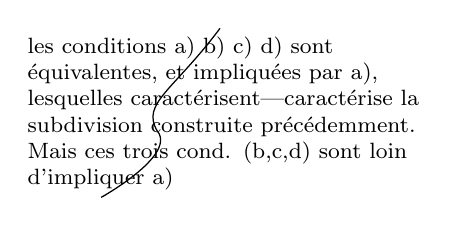
\begin{tikzpicture}[x=1cm,y=1cm]
\node[anchor=north west,inner sep=0pt,text width=5.0cm,align=left,font=\footnotesize] (longnote) at (0,0) {les conditions \deleted{\unsure{a)}} b) c) d) sont équivalentes, \unsure{et} \uline{impliquées} par a), lesquelles \unsure{caractérisent|caractérise} la subdivision construite précédemment. Mais ces trois \unsure{cond.} (b,c,d) sont \unsure{loin} d'impliquer a)};
\draw[line width=.45pt] ([xshift=2.45cm,yshift=.1cm]longnote.north west) .. controls (1.85,-.70) and (1.45,-.85) .. (1.65,-1.20) .. controls (1.95,-1.55) and (.65,-2.20) .. ([xshift=1.0cm,yshift=-.05cm]longnote.south west);
\end{tikzpicture}}}
% @ lower middle, condition b)
b) L'application can. associée à $F'\preceq F$
\[
 \varphi:F'\longrightarrow F
\]
induit une bijection
\[
 F'\setminus G'\xrightarrow{\sim}F\setminus G.
\]
% @ right, NB with a vertical left rule
\margin{\figure{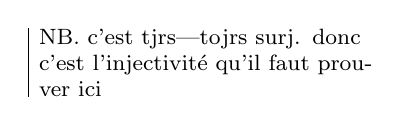
\begin{tikzpicture}
\node[anchor=north west,inner sep=0pt,text width=4.4cm,align=left,font=\footnotesize] (nb) at (0,0) {NB. c'est \unsure{tjrs|tojrs} surj. donc c'est l'\uline{injectivité} qu'il faut prouver ici};
\draw[line width=.4pt] ([xshift=-.13cm]nb.north west) -- ([xshift=-.13cm]nb.south west);
\end{tikzpicture}}}
% @ lower part, condition c), cancelled draft and interlinear replacement
c) \deleted{Les strates ouvertes de $F'$ qui ne sont} \inserted{$\forall A\in F\setminus G$, $A^\circ$ est une strate ouverte de $F'$.}
% @ lower part, condition d)
d) $F'\supset F\setminus G$, i.e. $\forall A\in F\setminus G$, on a $A\in F'$.

% @ foot, proof heading: one live On; no separate cancelled On is visible
\uline{Dém} On va prouver p. ex
\[
 \text{d)}\Longrightarrow\text{b)}\Longrightarrow\text{c)}\Longrightarrow\text{a)}\Longrightarrow\text{d)}
\]
% @ bottom, first implication and overwritten identity / inclusion
\deleted{\uline{Dém}} $\text{d)}\Rightarrow\text{b)}$ Si $(F\setminus G)\subset F'$, alors $\varphi\mid F\setminus G$ est l'\deleted{\unsure{identité}}\unsure{inclusion} \deleted{(trivial)} \inserted{can. $F\setminus G\hookrightarrow F$}, \deleted{donc} donc il reste à prouver
\[
 F\setminus G=F'\setminus G'.
\]
